\documentclass{scrarticle}
\usepackage[a4paper, total={6in, 10in}]{geometry}
\usepackage[ngerman]{babel}

\usepackage{xcolor}
\usepackage{graphicx}
\usepackage{multirow} % Wichtig: Fügen Sie dieses Paket in Ihrer Präambel hinzu!
\usepackage{array} % Oft nützlich in Verbindung mit tabularx

\usepackage{amsmath}
\usepackage{amsthm}
\usepackage{amssymb}
\usepackage{algorithm}
\usepackage[noend]{algpseudocode}

\usepackage{tikz}

\usepackage[colorlinks=true, linkcolor=black, citecolor=black, urlcolor=black]{hyperref}

\newtheorem{satz}{Satz}[section]
\newtheorem{lemma}{Lemma}[section]
\newtheorem{definition}{Definiton}[section]
\numberwithin{equation}{section}

\makeatletter
\renewcommand{\ALG@name}{Algorithmus}
\makeatother
\algrenewcommand\algorithmicrequire{\textbf{Eingabe:}}
\algrenewcommand\algorithmicensure{\textbf{Ausgabe:}}

\title{Metal-Oxide-Semiconductor Transistoren}
\author{Stephan Epp\\\texttt{hjstephan86@gmail.com}}
\date{\today}

\begin{document}
\maketitle
Metal-Oxide-Semiconductor (MOS) Transistoren bilden die Grundlage für hochintegrierte Schaltungen. Die U-I-Kennlinie eines nMOS-Transistors folgt in den verschiedenen Betriebsbereichen spezifischen mathematischen Formeln. Diese Formeln basieren auf physikalischen Modellen des Transistors und beschreiben den Drain-Source-Strom $I_{DS}$ in Abhängigkeit von den angelegten Spannungen. Diese bestehen hauptsächlich aus der Gate-Source-Spannung $U_{GS}$ und der Drain-Source-Spannung $U_{DS}$. Es gibt drei Hauptbetriebsbereiche für einen nMOS-Transistor: den Sperrbereich, den Triodenbereich und den Sättigungsbereich.

\section{Sperrbereich}
In diesem Bereich ist der Transistor ausgeschaltet und leitet praktisch keinen Strom.

\begin{itemize}
	\item \textbf{Bedingung:} $U_{GS} < U_{TH}$ (wobei $U_{TH}$ die Schwellenspannung ist).
	\item \textbf{Formel:}
	\begin{equation*}
		I_{DS} \approx 0
	\end{equation*}
	\item \textbf{Erklärung:} Wenn die Gate-Source-Spannung $U_{GS}$ unter der Schwellenspannung $U_{TH}$ liegt, kann sich kein leitender Kanal zwischen Source und Drain bilden, und es fließt kein nennenswerter Strom, d.h., $I_{DS} \approx 0$. Idealisiert ist $I_{DS} = 0$, in der Realität gibt es einen sehr kleinen Leckstrom (Subthreshold-Strom), der oft vernachlässigt wird.
\end{itemize}

\section{Triodenbereich / Linearer Bereich}
Dieser Bereich wird auch als ohmscher Bereich bezeichnet, da der Transistor hier wie ein spannungsgesteuerter Widerstand wirkt. Der Strom steigt hier nahezu linear mit $U_{DS}$ an (für kleine $U_{DS}$) und ist stark von $U_{GS}$ abhängig.

\begin{itemize}
	\item \textbf{Bedingung:} $U_{GS} > U_{TH}$ und $U_{DS} < (U_{GS} - U_{TH})$
	\item \textbf{Formel (vereinfachtes Modell für lange Kanäle):}
	\begin{equation*}
		I_{DS} = \mu_n C_{ox} \frac{W}{L} \left( (U_{GS} - U_{TH})U_{DS} - \frac{1}{2}U_{DS}^2 \right)
	\end{equation*}
	\begin{itemize}
		\item $\mu_n$: Elektronenbeweglichkeit im Kanal
		\item $C_{ox}$: Oxidkapazität pro Flächeneinheit
		\item $W$: Kanalbreite
		\item $L$: Kanallänge
		\item $U_{TH}$: Schwellenspannung
	\end{itemize}
	\item \textbf{Erklärung:} Wenn $U_{GS}$ über $U_{TH}$ liegt, bildet sich ein Kanal. Solange $U_{DS}$ nicht zu hoch ist, verhält sich der Kanal wie ein variabler Widerstand. Der Strom nimmt mit zunehmendem $U_{DS}$ zu und die Breite des Kanals verringert sich zum Drain hin leicht, was zu einer nicht-linearen Abhängigkeit führt, die durch den Term $U_{DS}^2$ beschrieben wird. Der nicht-lineare Anstieg vom gesperrten Zustand im Übergang bis in den leitenden Zustand bezieht sich auf den Übergang vom Sperrbereich in diesen Bereich und den anfänglich nicht-linearen Anstieg des Stroms, bevor er in die Sättigung geht.
\end{itemize}

\section{Sättigungsbereich}
In diesem Bereich verhält sich der Transistor wie eine spannungsgesteuerte Stromquelle, da der Drain-Source-Strom weitgehend unabhängig von $U_{DS}$ ist.

\begin{itemize}
	\item \textbf{Bedingung:} $U_{GS} > U_{TH}$ und $U_{DS} \ge (U_{GS} - U_{TH})$
	\item \textbf{Formel (vereinfachtes Modell für lange Kanäle):}
	\begin{equation*}
		I_{DS} = \frac{1}{2} \mu_n C_{ox} \frac{W}{L} (U_{GS} - U_{TH})^2 \left( 1 + \lambda U_{DS} \right)
	\end{equation*}
	\begin{itemize}
		\item Der Term $(1 + \lambda U_{DS})$ berücksichtigt den \textbf{Kanallängenmodulationseffekt}, $\lambda$ ist der Kanallängenmodulationsparameter, der eine leichte Zunahme des Stroms mit $U_{DS}$ in der Sättigung beschreibt. Ohne diesen Effekt wäre der Strom konstant.
	\end{itemize}
	\item \textbf{Erklärung:} Sobald $U_{DS}$ einen bestimmten Wert erreicht ($U_{DS,sat} = U_{GS} - U_{TH}$), wird der Kanal am Drain-Ende "abgeschnürt" (pinch-off). Eine weitere Erhöhung von $U_{DS}$ führt nicht zu einer signifikanten Zunahme des Stroms, da der Stromfluss durch die Anzahl der Ladungsträger im Kanal und die Gate-Spannung begrenzt wird.
\end{itemize}

\section{U-I-Kennlinie für $U_{GS} = 2\,\mathrm{V}$}

Für \( U_{GS} = 2\,\mathrm{V} \), \( U_{TH} = 0.2\,\mathrm{V} \) und \( k = 1\,\mathrm{mA/V^2} \) ergibt sich:
\begin{figure}[h]
	\centering
	\label{fig:kennlinie}
	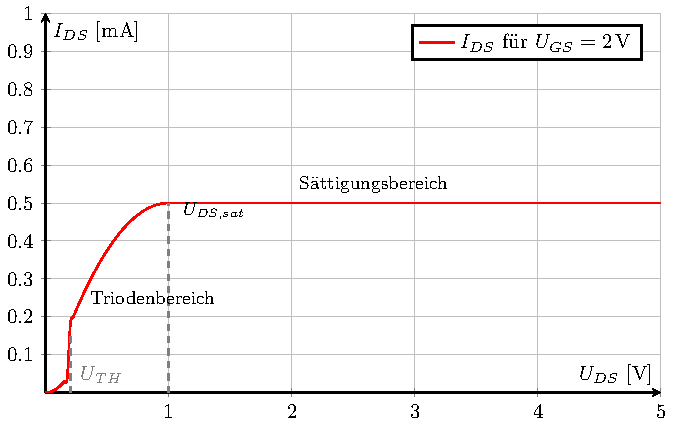
\includegraphics[scale=1.0]{tkiz/ui-kennlinie.pdf}
	\caption{U-I-Kennlinie eines nMOS-Transistors mit $U_{GS} = 2\,\mathrm{V}$}
\end{figure}
\begin{itemize}
	\item \textbf{Sperrbereich} ($U_{GS} < U_{TH}$, näherungsweise $U_{DS} < 0.2\,\mathrm{V}$): \\
	\[
	I_{DS} \approx a \cdot U_{DS}^2 \quad \text{mit } a = 1.25\,\mathrm{mA/V^2}
	\]
	\item \textbf{Triodenbereich} ($0.2\,\mathrm{V} < U_{DS} < 1\,\mathrm{V}$): \\
	\[
	I_{DS} = k \left((U_{GS} - U_{TH}) U_{DS} - \frac{1}{2} U_{DS}^2\right)
	\]
	\item \textbf{Sättigungsbereich} ($U_{DS} \ge 1\,\mathrm{V}$): \\
	\[
	I_{DS} = \frac{1}{2} k (U_{GS} - U_{TH})^2 = 0{,}5\,\mathrm{mA}
	\]
\end{itemize}

\section{Complementary Metal-Oxide-Semiconductor (CMOS)}
\label{sec:cmos}
Bevor der CMOS Schaltkreis betrachtet wird, wird das Schaltsymbol des pMOS-Transistors und das Schaltsymbol des nMOS-Transistors in Abbildung \ref{fig:pmos-nmos} gezeigt.
\begin{figure}[ht]
	\centering
	\begin{minipage}[t]{0.45\textwidth}
		\centering
		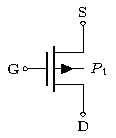
\includegraphics[scale=2.2]{tkiz/pmos.pdf}
	\end{minipage}
	\hfill
	\begin{minipage}[t]{0.45\textwidth}
		\centering
		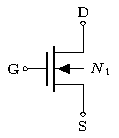
\includegraphics[scale=2.2]{tkiz/nmos.pdf}
	\end{minipage}
	\caption{Schaltsymbol des pMOS-Transistors $P_1$ und des nMOS-Transistors $N_1$}
	\label{fig:pmos-nmos}
\end{figure}

Complementary Metal-Oxide-Semiconductor (CMOS) Schaltkreise sind Schaltkreise, in denen der pMOS- und der nMOS-Transistor komplementär zueinander verbunden werden.
\begin{figure}[h]
	\centering
	\label{fig:cmos-not}
	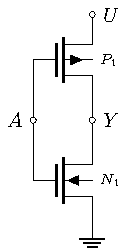
\includegraphics[scale=1.7]{tkiz/cmos-not.pdf}
	\caption{CMOS-Schaltung}
\end{figure}
Abbildung \ref*{fig:cmos-not} zeigt eine CMOS-Schaltung mit der Betriebsspannung $U$, der Eingangsspannung $A$ für die Transistoren $P_1$ und $N_1$ und der Ausgangsspannung $Y$. Dabei ist $P_1$ der pMOS-Transistor und $N_1$ der nMOS-Transistor.

Beim nMOS-Transistor $N_1$ zeigt der Pfeil auf den Transistor. Dies zeigt seine physikalische Wirkungsweise. Ist die Eingangsspannung $A$ ausreichend groß, dann liegt am Gate eine positive Spannung an. Das bewirkt wie beim Kondensator einen Feldeffekt zwischen den beiden Kondensatorplatten, der die Minoritäten (Elektronen) des nMOS-Transistors unter die Oberfläche der gegenüberliegenden Kondensatorplatte zieht. Erst durch diesen Feldeffekt tragen die Minoritätsladungsträger in ihrer Unterzahl im p-Substrat zum Stromfluss bei. Ist die Eingangspannung nämlich nicht ausreichend hoch, sperrt der nMOS-Transistor. Daher wird der nMOS-Transistor auch nMOS-Feldeffekttransistor (nMOSFET) genannt.

Beim pMOS-Transistor $P_1$ zeigt der Pfeil weg von der unteren Kondensatorplatte. Das liegt daran, dass die Elektronen im pMOS-Transistor nicht Minoritätsladungsträger sondern Majoritätsladungsträger sind. Das heißt, der pMOS-Transistor leitet sogar schon bei einer Eingangsspannung von $A = 0\mathrm{V}$. Der Feldeffekt beim pMOS-Transistor führt dazu, dass bei ausreichender Eingangsspannung $A$ am Gate die Minoritätsladungsträger im n-Substrat unter die Kondensatorplatte gezogen werden und der pMOS-Transistor sperrt. Daher wird der pMOS-Transistor auch pMOS-Feldeffekttransistor (pMOSFET) genannt.

Beide Transistoren $P_1$ und $N_1$ in Reihe geschaltet haben somit ein physikalisch komplementäres Sperr- und Leitverhalten zueinander. Dieses komplementäre Sperr- und Leitverhalten gibt diesem Schaltkreis den Namen Complementary Metal-Oxide-Semiconductor (CMOS) Schaltkreis.

Betrachtet man das logische Schaltverhalten der CMOS Schaltung in Abhängigkeit der Betriebsspannung $U$, der Eingangsspannung $A$ und der Ausgangsspannung $Y$, wird klar, dass mit dieser Schaltung ein Inverter betrieben wird. Ist $A = 0$, leitet $P_1$ und $N_1$ sperrt. Das heißt, das Bezugspotenzial für $Y$ ist $U$ und damit ist $Y = 1$ (Pull-Up-Bezugspotenzial). Ist $A = 1$, sperrt $P_1$ und $N_1$ leitet. Das heißt, das Bezugspotenzial für $Y$ ist die Masse und damit ist $Y = 0$ (Pull-Down-Bezugspotenzial).

\section{Logische Gatter: NND und NOR}
Ein logisches Gatter (oft auch einfach Gatter oder englisch (logic) gate genannt) ist ein grundlegender Baustein in der digitalen Elektronik, der eine bestimmte boolesche Funktion berechnet.
\begin{figure}[ht]
	\begin{minipage}[t]{0.5\textwidth}
		\centering
		\begin{tabular}{c|c||c}
			\hline
			$A$ & $B$ & $A \text{ NND } B$ \\
			\hline\hline
			0 & 0 & 1 \\
			0 & 1 & 1 \\
			1 & 0 & 1 \\
			1 & 1 & 0 \\
			\hline
		\end{tabular}
	\end{minipage}
	\hfill % Sorgt für horizontalen Abstand zwischen den minipages
	\begin{minipage}[t]{0.5\textwidth}
		\centering
		\begin{tabular}{c|c||c}
			\hline
			$A$ & $B$ & $A \text{ NOR } B$ \\
			\hline\hline
			0 & 0 & 1 \\
			0 & 1 & 0 \\
			1 & 0 & 0 \\
			1 & 1 & 0 \\
			\hline
		\end{tabular}
	\end{minipage}
	\caption{Boolesche Funktion NND und NOR}
\label{fig:nand-nor}
\end{figure}
In Kapitel \ref{sec:cmos} wird ein Inverter beschrieben, der die boolesche Funktion des NOT Gatters in Abhängigkeit des Eingangssignals $A$ berechnet. Andere Gatter, die durch CMOS-Schaltungen gebildet werden können, sind das NAND (kurz: NND) Gatter und das NOR Gatter. Das NND Gatter und das NOR Gatter bilden boolesche Funktionen in Abhängigkeit der Eingangssignale $A$ und $B$. Abbildung \ref{fig:nand-nor} zeigt die vollständig beschriebene boolesche Funktion beider Gatter. Dadurch, dass diese booleschen Funktionen durch MOSFETs gebildet werden können, sind ihre Funktionen als Hardwarelösung jeweils in einem Takt eines Prozessors berechenbar. In einem Takt würde ein Prozessor das Programm, das z.B. die boolesche NND Funktion als Softwarelösung berechnet, nicht berechnen können.


\end{document}